\documentclass{article}
\usepackage{graphicx} % Needed for including graphics.
\usepackage{amsmath}  % Needed for math features.

\title{Designing an Efficient Interpolation Method}
\author{ByeongKyu Park}
\date{\today}

\begin{document}
\maketitle
\section{The Idea}
This method introduces a practical approach to data interpolation by combining slope-based segmentation with Lagrange polynomial interpolation within each segment. Unlike some traditional interpolation techniques that require complex computations or rely heavily on derivative information, this strategy segments data according to changes in slope, then interpolates those segments individually. This approach aims to more naturally represent data trends, especially in large datasets, by avoiding some common pitfalls of high-degree polynomial interpolation, such as Runge's phenomenon.

\section{The Computation}
Our method for interpolating data involves a straightforward sequence of steps that prioritize mathematical simplicity and computational efficiency. Below is a detailed explanation:

\begin{enumerate}
    \item \textbf{Slope Calculation and Trend Identification:} 
    The initial step involves calculating the slope between each pair of adjacent points to determine the immediate direction in which the data is moving, be it upward, downward, or remaining constant. For points $(x_i, y_i)$ and $(x_{i+1}, y_{i+1})$, the slope is calculated as $\frac{y_{i+1} - y_i}{x_{i+1} - x_i}$. 

	\item \textbf{Classification and Propagation:} 
After the slopes between consecutive points are calculated, we determine the trend shifts by examining the forward differences of these slopes. Each segment between points is initially classified as positive (+), negative (-), or neutral (0) based on its slope. To refine the classification and achieve a consistent trend representation, particularly when direct slope calculations result in zeros, we adjust these neutral classifications to match the trend of the immediately preceding segment. This step ensures segments with initially unclear trends are aligned with the broader, contiguous trend they are part of.

	\textbf{Example:}
Consider a dataset resulting in calculated slopes between points represented by the sequence $[1, 0, 0, -1, 0]$. This sequence leads to an initial trend classification of $[+, 0, 0, -, 0]$, where + indicates an increasing trend, - a decreasing trend, and 0 a stable or unclear trend. For segments classified as 0, we adjust their classification based on the trend of the adjacent segment to their left. Therefore, the sequence $[+, 0, 0, -, 0]$ is updated to $[+, +, +, -, -]$ after propagation. This adjustment reflects a more coherent analysis of the dataset's trend, ensuring that segments initially classified as stable or unclear are correctly interpreted within the context of their neighboring trends. Such refinement is pivotal for the precise application of Lagrange polynomial interpolation to each segmented part of the dataset.



\end{enumerate}


\section{The Results}
Below are the interpolated results for the given \(x, y\) values.

\begin{figure}[htbp]
\centering
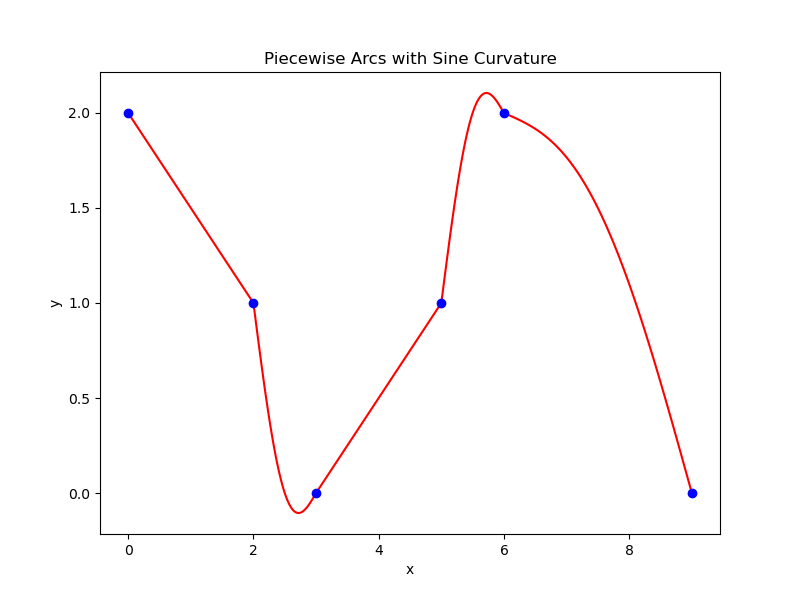
\includegraphics[width=0.8\textwidth]{test_case_1.png}
\caption{Interpolation on Dataset 1}
\end{figure}

\begin{figure}[htbp]
\centering
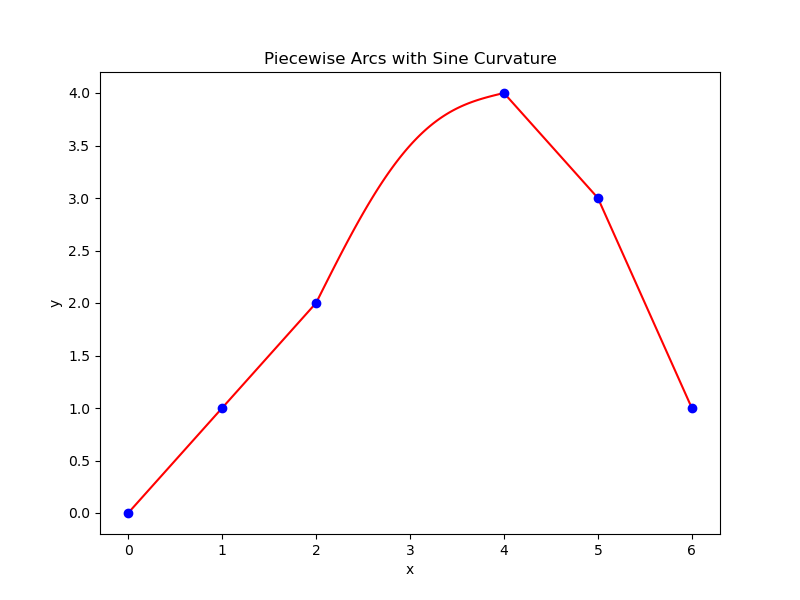
\includegraphics[width=0.8\textwidth]{test_case_2.png}
\caption{Interpolation on Dataset 2}
\end{figure}

\begin{figure}[htbp]
\centering
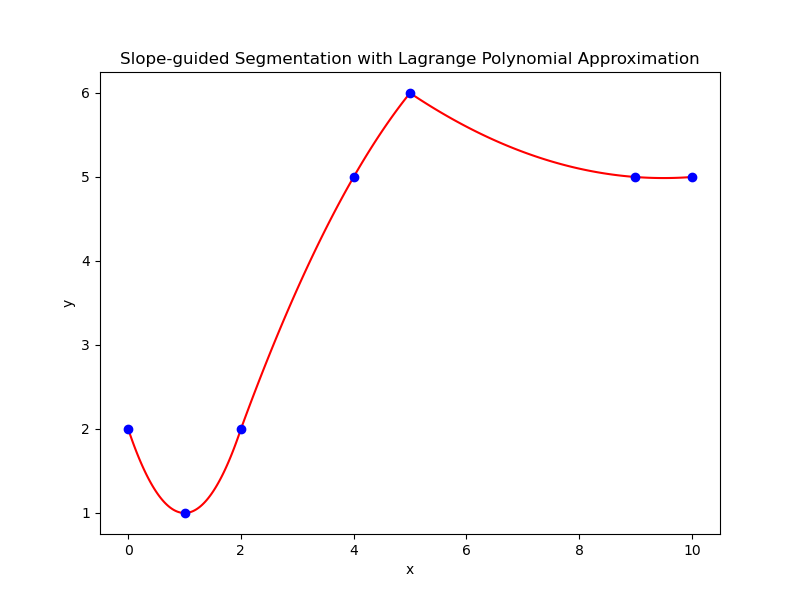
\includegraphics[width=0.8\textwidth]{test_case_3.png}
\caption{Interpolation on Dataset 3}
\end{figure}

\begin{figure}[htbp]
\centering
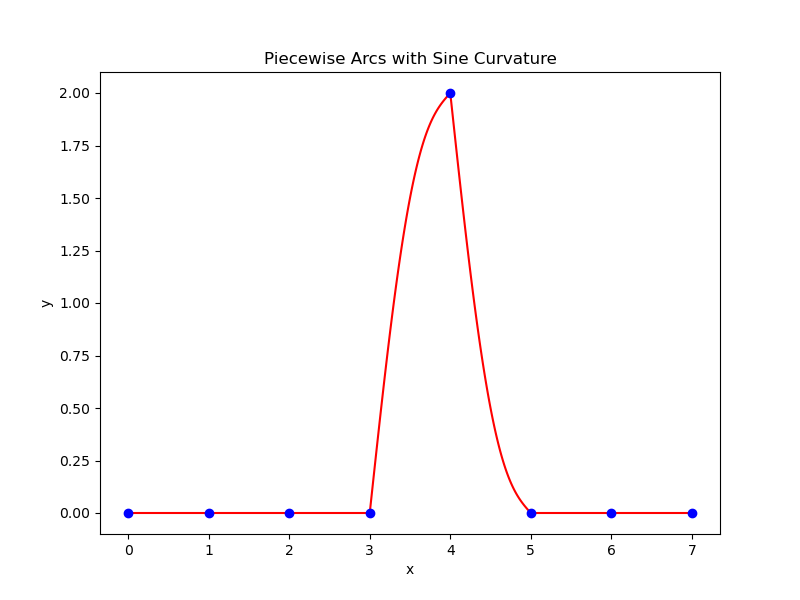
\includegraphics[width=0.8\textwidth]{test_case_4.png}
\caption{Interpolation on Dataset 4}
\end{figure}

\begin{figure}[htbp]
\centering
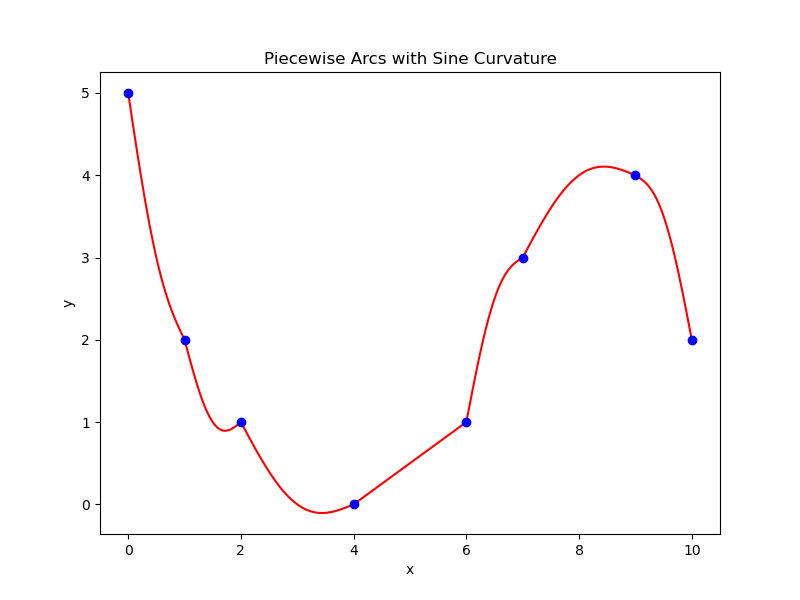
\includegraphics[width=0.8\textwidth]{test_case_5.png}
\caption{Interpolation on Dataset 5}
\end{figure}

\newpage
\section{Possible Issues}
While our method is designed to simplify the interpolation process and improve efficiency, it does face some inherent limitations:

\begin{enumerate}
    \item \textbf{Vulnerability to Runge's Phenomenon Despite Reduced Points:} 
    By segmenting the data and applying Lagrange polynomial interpolation to smaller sets of points, we aim to mitigate the risk of oscillatory behaviors typical of high-degree polynomial interpolations. However, this method is not entirely immune to Runge's phenomenon. Even with fewer points per segment, interpolating polynomials can still exhibit unwanted oscillations, especially near the edges of each segment or when segments consist of widely spaced points.
    
    \item \textbf{Order Sensitivity in Differentiation:} 
    The direction of computation notably impacts the outcome, particularly evident when calculating forward differences for slope and trend identification. This order sensitivity can lead to varying segmentations of the dataset, subsequently affecting the interpolated curves' consistency. Different computational directions may yield distinct interpretations of the same data, posing a challenge for achieving a uniformly accepted interpolation result.
\end{enumerate}

\section{Possible Extensions}
To further refine the approach and address its limitations:
\begin{enumerate}
    \item Adaptive curvature adjustments could be explored to more accurately represent data with rapid directional changes or nuanced variations, potentially by altering segment curvatures based on detailed trend analysis.
    \item Incorporating alternative interpolation techniques, such as spline interpolation, within segments might offer smoother transitions and mitigate the effects of Runge's phenomenon.
    \item A deeper investigation into the impact of differentiation order on segmentation could yield insights leading to adjustments in the algorithm that account for directional biases.
\end{enumerate}

\end{document}
